\title{Using shotgun metagenomic data for SSU rRNA gene community analysis}
\author{}

\documentclass[12pt]{article}
\usepackage[a4paper, margin=1in]{geometry}
\usepackage[parfill]{parskip}

% set double space
\usepackage{setspace}
\doublespacing

% set times fond
\usepackage{times}

% line number index
\usepackage{lineno}
\linenumbers

% Compile only with pdfLaTeX
\usepackage[pdftex]{graphicx}

\begin{document}
\maketitle

\begin{abstract}
  Amplicon sequencing of SSU rRNA genes amplified directly from environmental sample DNA extractions is now standard procedure for assessing microbial community structures. In contrast, metagenomic shotgun sequencing does not depend on gene-targeted primers or PCR amplification and thus is not affected by primer bias or chimeras, respectively. However, it is difficult to detect and recover SSU rRNA genes from shotgun data and then to analyze them because of the large number and short lengths of the reads. A framework (SSUsearch, or need a better name; it’s not about search anymore;  MG-RNA, SG-RNA, RNAlyze?) was developed to search for the SSU rRNA gene fragments in shotgun data followed by supervised classification, clustering, copy correction and operational taxonomy unit (OTU) based diversity analysis. Taxonomy profile comparison of shotgun data and amplicon data from the same sample shows bias against Actinobacteria and Verrucomicrobia in the V6-V8 primer set and Actinobacteria in the V4 primer. Besides taxonomy based diversity analyses, this pipeline also enabled {\em de novo} OTU based diversity analyses. In application to rhizosphere soil samples, shotgun metagenomic data show higher diversity than amplicon data but the same grouping of samples in ordination analyses. Firmicutes have highest fold change after copy correction in both soil samples. The HMM model can recover Bacteria, Archaea and Eukaryota. Further, the analysis framework can be applied to LSU rRNA providing additional confirmation of community structure.
\end{abstract}

\section{Introduction}
  Microorganisms are distributed in all four domains in the tree of life and recognized for their key roles in ecosystem processes, in many nutrient recycling and industrial processes and in the health or disease of higher organisms. They are highly diverse at genetic level because of their ancient history and habitat diversity (\cite{ward2002}). It is well known that most of them have not been cultured, which has become especially clear with the advent of sequencing of SSU rRNA from environmental samples. The high-throughput sequencing technologies such as pyrosequencing (454) and Illumina sequencing (MiSeq) of short hyper-variable regions of a phylogentic marker gene, ribosomal Small Subunit (SSU rRNA) gene, provide means of accessing the uncultured majority (\cite{streit2004}). Although with the disadvantange of primer bias, these high-throughput technologies (also called amplicon sequencing due to PCR amplification of targeted gene) have been extensively used in community structure surveys and renewed our understanding of microbial diversity from many environments (\cite{huse2008,caporaso2012miseq}). Meanwhile, the growing databases of SSU rRNA genes provide a rich ecological and phylogenetic context for SSU rRNA gene based community structure surveys (\cite{rdp2009,silva2013}).

  Unlike gene targeted amplicon sequencing, shotgun sequencing should provide a more accurate characterization of microbial diversity because it eliminates primer bias and chimera by sequencing randomly sheared fragment of metagenome (\cite{chimeraslayer}), though it is still prone to sequencing error and any bias from environmental DNA extraction. Thus it provides an improved means to detect divergent sequences not recovered by standard SSU rRNA gene primers, such as for Verrucomicrobia as well as the eukaryotic members of the community (\cite{baker2003,primereva2008,verruco2011}).

  The challenges for use of shotgun DNA for SSU rRNA analyses are the efficient search for these fragments and, more so, the subsequent analysis because of the short reads. Several methods have been developed for fast SSU rRNA retrieval in large data sets (\cite{ribopicker,metarna,rrnaselector,metaxa}), but none of them provides further community analysis using the identified rRNA gene sequences, which is of great interest in the field of microbial ecology due to less bias shotgun metagenome. On the other hand, traditional community analysis tools (\cite{rdp2009,mothur,qiime}) are mainly designed to handle amplicon sequences that are amplified by PCR primers. There are two types of traditional community analyses: reference based and OTU based. The reference based method assigns SSU rRNA gene sequence to bins based on taxonomy of its closest reference sequences and OTU based method assigns gene sequences to bins based on de-novo clustering with certain similarity cutoff (usually 97\%). The reference based method can applied to shotgun data easily once SSU rRNA gene fragments are found by assigning taxonomy (\cite{rdpclassifier}), while OTU based method is not that straightforward on shotgun data.

  The main goal of this study is to enable both OTU based and reference based community analysis in shotgun metagenome. First, Hidden Markov Model (HMM) based methods already shown to be fast and accurate for SSU rRNA search (\cite{metarna,rrnaselector,metaxa}) are applied with well-curated and updated training reference sequences from SILVA. Next analyzing step leverages the longer reads assembled from overlapping paired end reads and the deep coverage provided by Illumina shotgun sequencing and makes traditional OTU analyses applicable on reads mapped to small hyper-variable regions (150bp) of SSU rRNA genes. This analysis framework can also be extended to other genes. The ribosomal large subunit (LSU) gene, another phylogenetic marker on the same rrn operon as the SSU gene, is also analyzed with the same method and provides confirmatory analyses. We tested the framework on soil samples, arguably the most diverse communities and find several interesting differences between amplicon and shotgun.

\section{Materials and Methods}
  {\bf Soil sampling, DNA extraction and sequencing. }
Rhizosphere soil was sampled by collecting soil tightly attached (within 2mm) of roots and bulk soil was sampled obtained from the mid-point between plant rows. DNA extraction and SSU rRNA gene amplification was previously described (\cite{ed2010}). An SSU rRNA gene primer set (926F: AAACTYAAAKGAATTGACGG 1392R: ACGGGCGGTGTGTRC) was used target V6-V8 variable region in the standard Joint Genome Institute (JGI) 454 GS FLX and Titanium sequencing workflow and cover bacteria, archaea and eukaryotes (16S and 18S rRNA). Another primer set (515F: GTGCCAGCMGCCGCGGTAA 806R: GGACTACHVGGGTWTCTAAT) was used to target V4 variable region in JGI MiSeq sequencing workflow. Shotgun sequencing is done with Illumina GAII platforms and HiSeq using 250bp insert libraries and pair end 150bp read length. One switchgrass bulk soil sample (SB1) is sequenced by 454 Titanium and Illumina GAII platform. Seven replicates of corn (C1 - C2) and miscanthus (M1 - M2) rhizosphere soil samples are sequenced by MiSeq and HiSeq platform. All these samples are collected from GLBRC intensive site at  Kellog Biological Station, MI.

  {\bf Data preprocess. }
  The whole analysis framework is shown in Figure ~ref{fig:flowchart}. Data preprocess is necessary for both shotgun and amplicon data due to sequencing error. Trailing bases with quality score ``2'' endcoded by ASCII 66 ``B'' are trimmed off GAII Illumina 1.5 shotgun data and reads shorter than 30bp and with Ns are discarded using a python script. HighSeq shotgun data were quality trimmed with fast-mcf in the EA-Utils (http://code.google.com/p/ea-utils) with flags `` -l 50 -q 30 -w 4 -k 0 -x 0 --max-ns 0 -H''. Then paired-end reads with overlaps more than 10bp were assembled into one long read by FLASH (\cite{flash2011}) with ``-m 10 -M 120 -x 0.20 -r 140 -f 250 -s 25 -t 1''. 454 pyrotag amplicon data was processed using the RDP pyrosequencing pipeline (\cite{rdp2009}). Since the targeted region is about 467bp (926F/1392R), the reads were not long enough to cover the whole region, so only the reverse primer was used for quality trimming. The minimum length was set to 400bp and defaults were used for other parameters.

  {\bf Building SSU and LSU rRNA gene models. }
First, SILVA (\cite{silva2013}) SSU and LSU Ref NR database (version 115) sequences are quality trimmed to discard all sequences with ambiguous DNA bases and ``U'' is converted to ``T'', and then are clustered at 97\% similarity cutoff using pick\_otus.py and pick\_rep\_set.py in QIIME(\cite{qiime}). Then the longest representative in each OTU is chosen and further clustered at 80\% similarity cutoff. The longest sequence in each OTU is collected, resulting in 4027 representative sequences for SSU rRNA gene and 1295 for LSU as a phylogentically diverse set of reference genes. These sequences were further grouped into two groups, one with Bacteria and Archaea and the other with Eukaryota. Each group were then used to make a HMM (Hiden Markov Model) by hmmbuild in HMMER version 3.1 (\cite{hmmer3}) and two HMM files were concatenated as a single file.

  {\bf Identification of SSU and rRNA gene fragments from metagenomic data. }
  LSU and SSU HMM model were used to search against 1 lane of GAII Illumina shotgun reads from a bulk soil metagenome by hmmsearch in HMMER (version 3.1). Reverse complements of all reads were added to the shotgun sequence file before the hmmsearch. The HMMER hits using default e-value cutoff of 10 are fed into the multiple sequence aligner (align.seqs) implemented in Mothur (\cite{mothuraligner2009}). For SSU rRNA gene fragments, 18491 full-length SSU rRNA gene sequences (14956 from Bacteria, 2297 from Archaea, and 1238 from Eukaryota) from the SILVA database (\cite{silva2013}) provided in mothur website are used as template with flags ``search = suffix, threshold = 0.5, and filp = t''.  For LSU rRNA, Multiple Sequence Alignment (MSA) of representative sequences of SILVA LSU Ref NR database clustered at 97\% similarity cutoff is used as template with the same flags as SSU. Based on the detailed alignment information in report file, those shotgun reads with more than 50\% of their basepairs mapped to a reference gene are designated as SSU rRNA or LSU rRNA gene fragments. The results of SSU rRNA search are compared with BLAST (\cite{blast}) results. The representative sequences for making HMM are used to BLAST against the shotgun data with a e-value cutoff of $10^{-5}$.

  {\bf Comparison of taxonomy based microbial community structures inferred from shotgun and amplicon SSU rRNA gene sequences. }
The SSU rRNA fragments from shotgun data and amplicon data were classified using RDP’s Classifier (\cite{rdpclassifier}). The reference SSU rRNA genes from RDP and SILVA are provided in Mothur website and are used as the template and the bootstrap confidence cutoff for classification is 50\%. Meanwhile, representative sequences of SILVA Ref NR clustered at 97\% similarity cutoff are used as template and the taxonomy information can be extracted from the sequence file. The bacterial taxonomy profiles from shotgun data and amplicon data were compared at phylum level.

  {\bf Copy correction. }
  SSU rRNA gene copy number of each taxon in Greengenes database has previously been calculated (\cite{copyrighter}). In taxonomic summary, the abundance of each taxon is weighted by the inverse of its SSU rRNA gene copy number. Similarly in OTU based analysis, the abundance of each OTU is weighted by the inverse of SSU rRNA gene copy number of its taxon.

  {\bf Community structure comparison based on OTUs clustered from 150 hyper variable regions. }
  For the clustering analysis of shotgun and amplicon data, 150bp in V8 region (E.coli positions: 1227-1377) were aligned. Reads longer than 100bp were kept in the MSA of V8 region and then clustered by mcclust with minimum overlap of 25bp (\cite{rdp2009}). The clustering result was converted to Mothur format and beta diversity analysis was done by make.shared with ``label=0.03'', dist.shared(calc=thetayc), and pcoa command in Mothur. When comparing different regions, E. coli positions: 127-277, 577-727, and 997-1147 were chosen for V2, V4, and V6, respectively. The procrustes analysis provided in QIIME [Error! Reference source not found.qiime] was used. The PCoA results are plotted in the same figure; V2, V4 and V6 are transformed to minimize the distances between corresponding points in V8.

  {\bf Comparison of OTU based microbial community structures inferred from shotgun and amplicon SSU rRNA gene sequences. }
Abundance of each OTU in shotgun data and amplicon data (V6-V8 for SB1 and V4 for M1) from the same DNA extraction are compared to check the consistency between two types of sequencing technology. Pearson’s correlation coefficient and $R^2$ of linear regression are used to evaluate the correlation between two types of data and also correlation between two technical replicates. All the abundances of each OTU are increased by one to order to be displayed in log scale (avoiding zeros). There are 6 technical replicates (lanes) for SB1. We pooled first three as SB1\_123 and the others as SB1\_456 to achieve better sequencing depth.

\section{Results}
  {\bf Identification of SSU rRNA gene fragments in pair end shotgun data. }
  15566  (0.03\%) of out 44787632 quality trimmed and pair end merged sequences are identified as SSU rRNA fragments. The number is consistent with the BLAST search results (Figure ~\ref{fig:vennPlusIdenDisWholeLength}). We get longer sequences after merging overlapping pair ends shown in the peak between 150 and 300 bp in Figure ~\ref{fig:read_length_dist}. 
  *** compare with meta-rna instead of blast.

    \begin{figure}[tbph!]
    \centering
    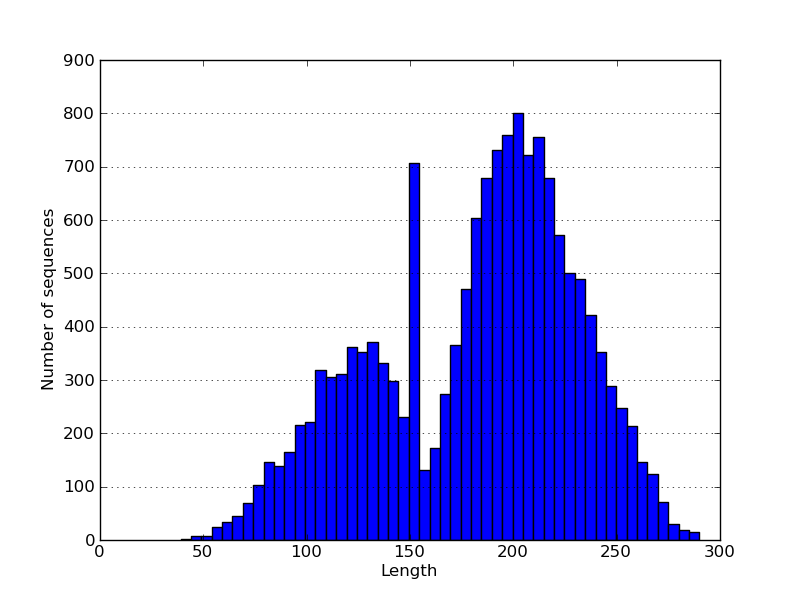
\includegraphics[width=0.8\textwidth]{figs/read_length_dist.png}
    \caption[Length distribution of identified SSU rRNA gene shotgun fragments]{Length distribution of identified SSU rRNA gene shotgun fragments. The peak with longer length results from the merged pair ends and benefits classification and {\em de novo} clustering in downsteam analyses.}
    \label{fig:read_length_dist}
    \end{figure}

  {\bf Comparison of taxonomy based microbial community structures inferred from shotgun and amplicon SSU rRNA gene sequences. }
The RDP Classifier can classify short fragments ($>50$bp) of SSU rRNA genes at the phylum level with high accuracy (RDP classifier). Both shotgun and amplicon data show Actinobacteria, Proteobacteria and Acidobacteria as the three most abundant phyla and take up about 70\% of community. More sequences are unclassified in shotgun data than in amplicon data. RDP and SILVA show consistent classification results. However, the 926F/1392R (V6-V8) primer set has bias against Verrucomicrobia, and the 515F/806R (V4) primer set has bias against Actinobacteria.

  To take advantage of the fact that shotgun data contain all genome fragments, the retrieved Large Subunit (LSU) rRNA genes on the same operon (rrn) as SSU rRNA gene were also classified. Their taxonomy profile is similar to that of SSU rRNA gene (Pearson’s correlation coefficient is 0.87 for SB1 and 0.91 for M1), except that more reads (19.6\%) are not classified. This is expected because of the much lower number of reference LSU rRNA genes in SILVA database. The two genes show consistent community profile at Bacterial phylum level and also confirm bias of primers. Further, both LSU and SSU HMM show the ability to identify the Eukaryotic members and gives about the same taxonomy profile at domain level.

\begin{figure}[tbph!]
  \centering
  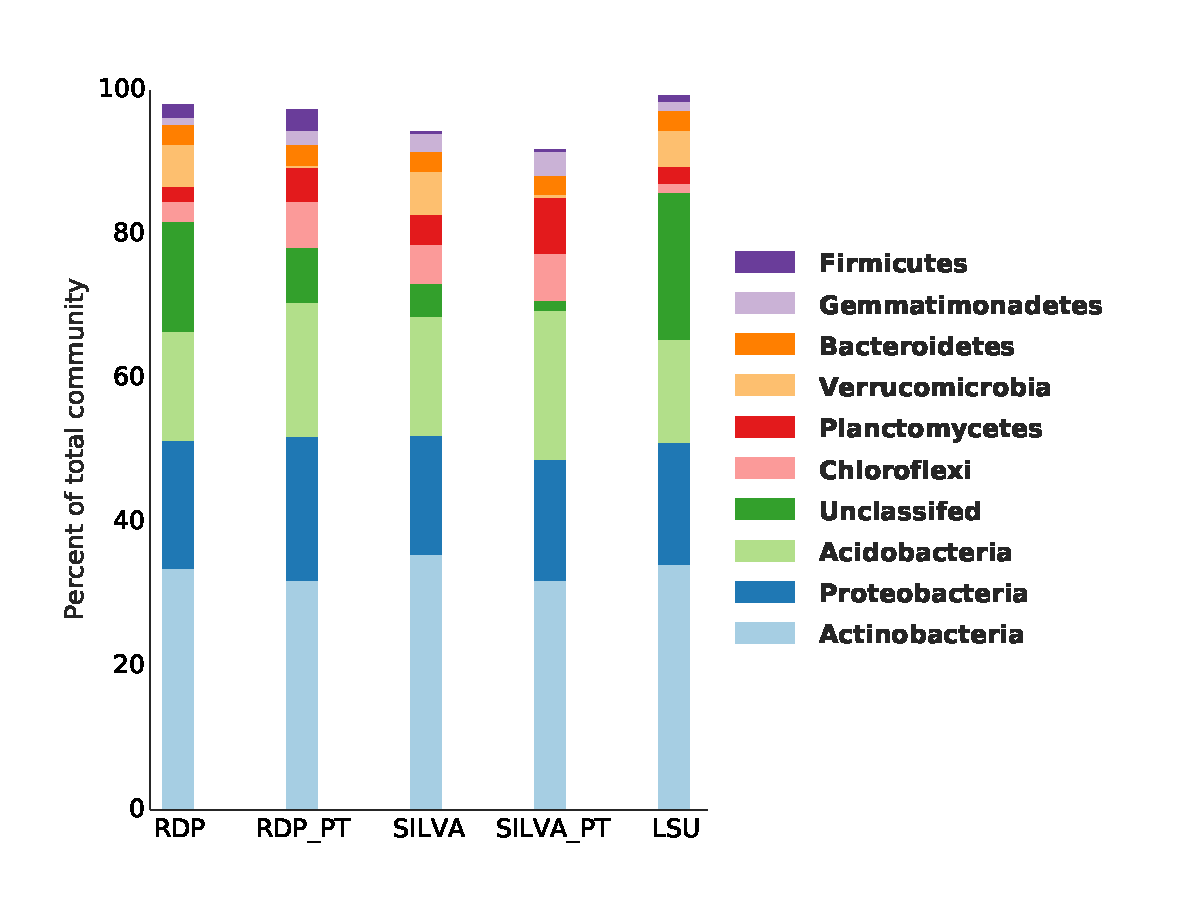
\includegraphics[width=0.8\textwidth]{figs/V6to8_SB1_taxa}
  \caption[Taxonomy profiles at Bacterial phylum level of shotgun fragments and of amplicon reads amplified using V6-V8 primer]{Taxonomy profiles at Bacterial phylum level of shotgun fragments from SSU and LSU rRNA gene and of amplicon reads amplified using V6-V8 primer (515F/806R). Classifications are done using both RDP and SILVA reference database. Amplicon data shows less Actinobacteria in both databases.}
  \label{fig:V6to8_SB1_taxa}
\end{figure}

\begin{figure}[tbph!]
  \centering
  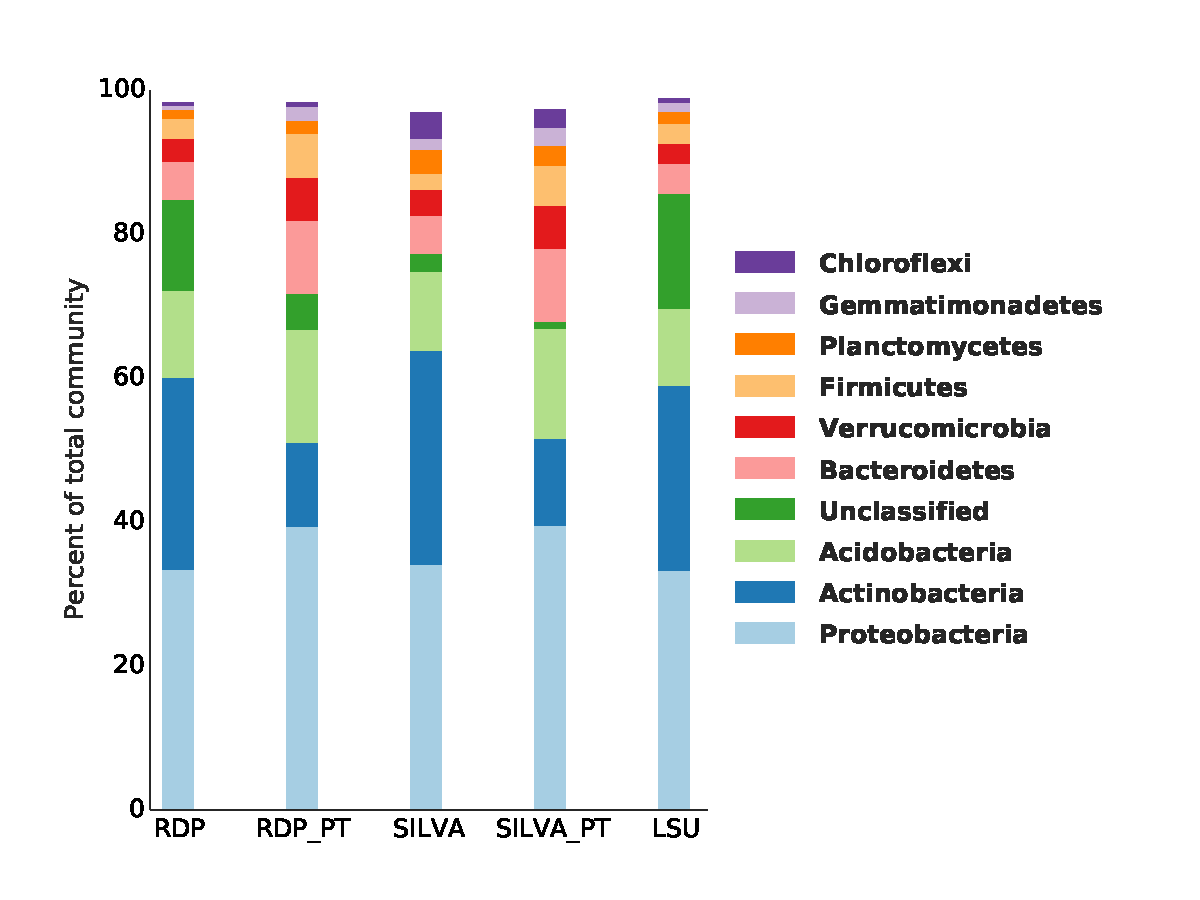
\includegraphics[width=0.8\textwidth]{figs/V4_M1_taxa}
  \caption[Taxonomy profiles at Bacterial phylum level of shotgun fragments  and of amplicon reads amplified using V4 primer]{Taxonomy profiles at Bacterial phylum level of shotgun fragments from SSU and LSU rRNA gene and of amplicon reads amplified using V4 primer (515F/806R). Classifications are done using both RDP and SILVA reference database. Amplicon data shows less Actinobacteria in both databases.}
  \label{fig:V4_M1_taxa}
\end{figure}

\begin{figure}[tbph!]
  \centering
  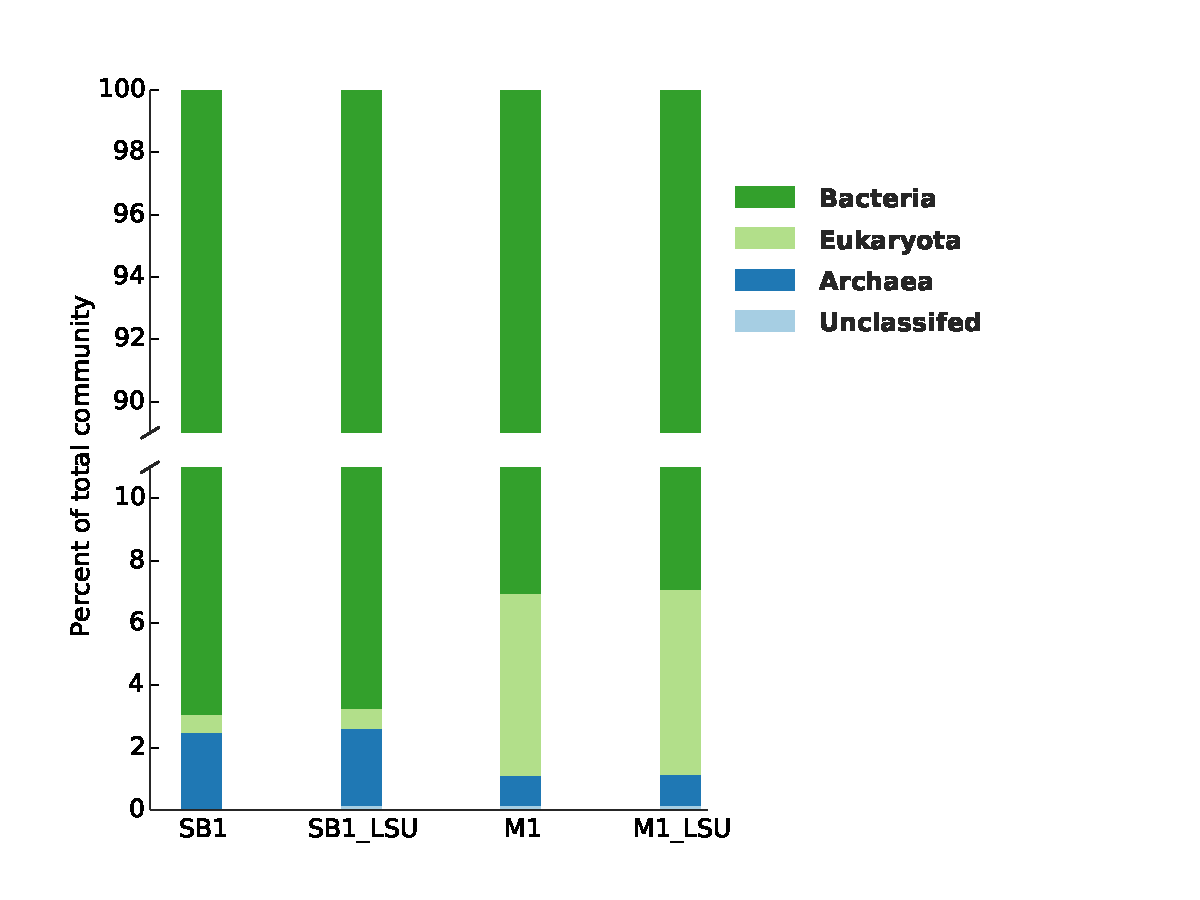
\includegraphics[width=0.8\textwidth]{figs/LSU_domain_taxa}
  \caption[Taxonomy profile at domain level using SILVA SSU and LSU rRNA database]{Supp. Taxonomy profile at domain level using SILVA SSU and LSU rRNA database. For both samples (SB1 and M1), SSU and LSU show consistent domain level taxonomy distribution (Pearson’s correlation coefficient = 1).}
  \label{fig:LSU_domain_taxa}
\end{figure}


  {\bf Comparison of OTU based microbial community structures inferred from shotgun and amplicon SSU rRNA gene sequences. }
  Figure ~\ref{fig:SB1_techrep_OTUscat} shows our analysis pipeline has good reproducibility between two technical replicates (Pearson’s correlation coefficient = 0.997). Even with log-transformed abundance, the two replicates have Pearson’s correlation coefficient of 0.91 and linear regression $R^2$ of 0.88. However, OTU abundance in shotgun and amplicon data does not correlate as well with Pearson’s correlation coefficient of 0.873 in SB1 and 0.581 in M1. There are OTUs with significant difference in shotgun data and amplicon data.

\begin{figure}[tbph!]
  \centering
  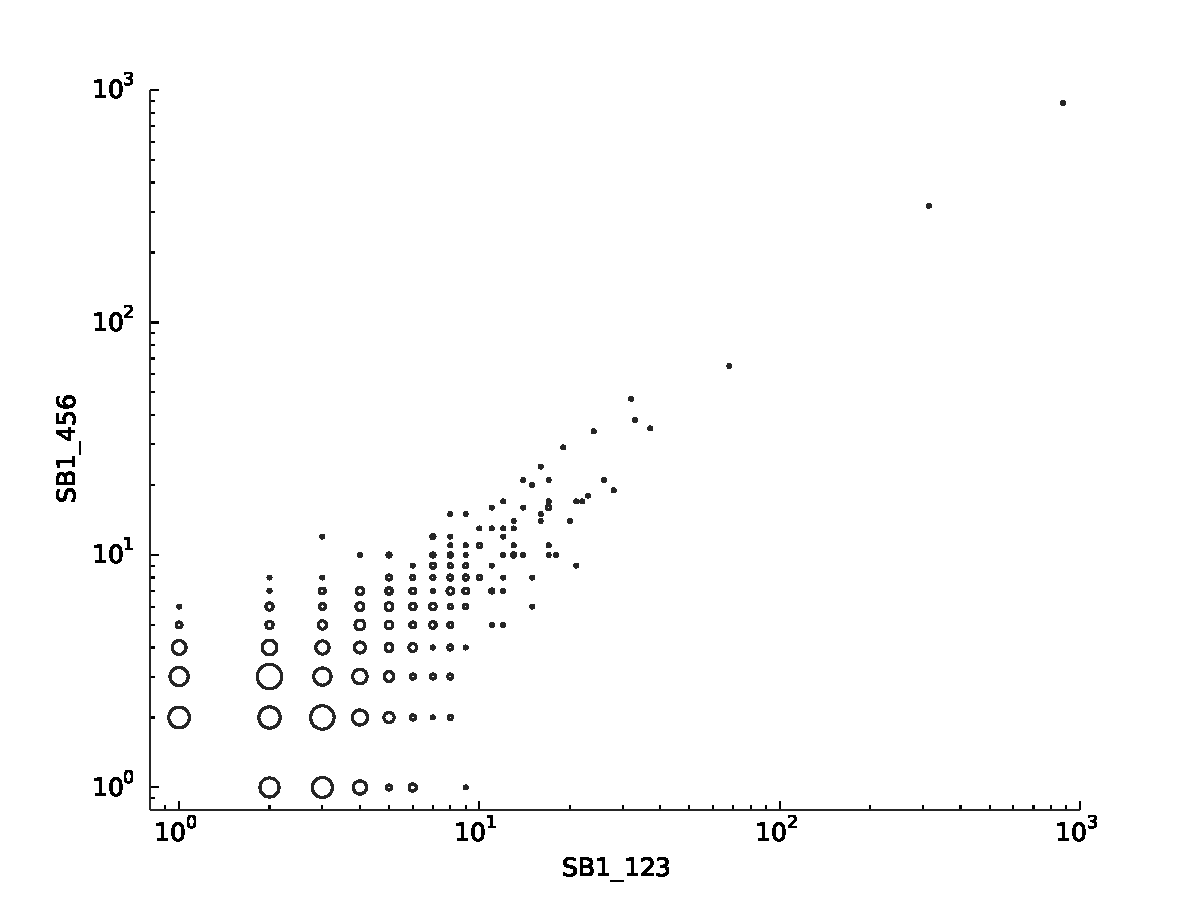
\includegraphics[width=0.8\textwidth]{figs/SB1_techrep_OTUscat}
  \caption[Technical reproducibilty test]{Supp. Technical reproducibility test. X axis shows number of raw reads per OTU in log scale in replicate SB1\_123, and y axis shows number of raw reads per OUT in log scale in replicate SB1\_456. The size of circle is proportional to number of OTUs with the same counts in SB1\_123 and also in SB1\_456. The counts are in both replicates are increased by 1 to avoid 0 counts that can be displaced in log scale. There are 6 techinical replicates for sample SB1 sequenced in 6 lanes of Illumnia plate using DNA from the same extraction. First three lanes are pooled as SB1\_123 and next three lanes are pooled as SB1\_456. The two technical replicates show consistent counts for each OTU, and the consistency is higher when the abundance of OTUs are higher. Pearson’s correlation coefficient is 0.997 on the original counts.}
  \label{fig:SB1_techrep_OTUscat}
\end{figure}

\begin{figure}[tbph!]
  \centering
  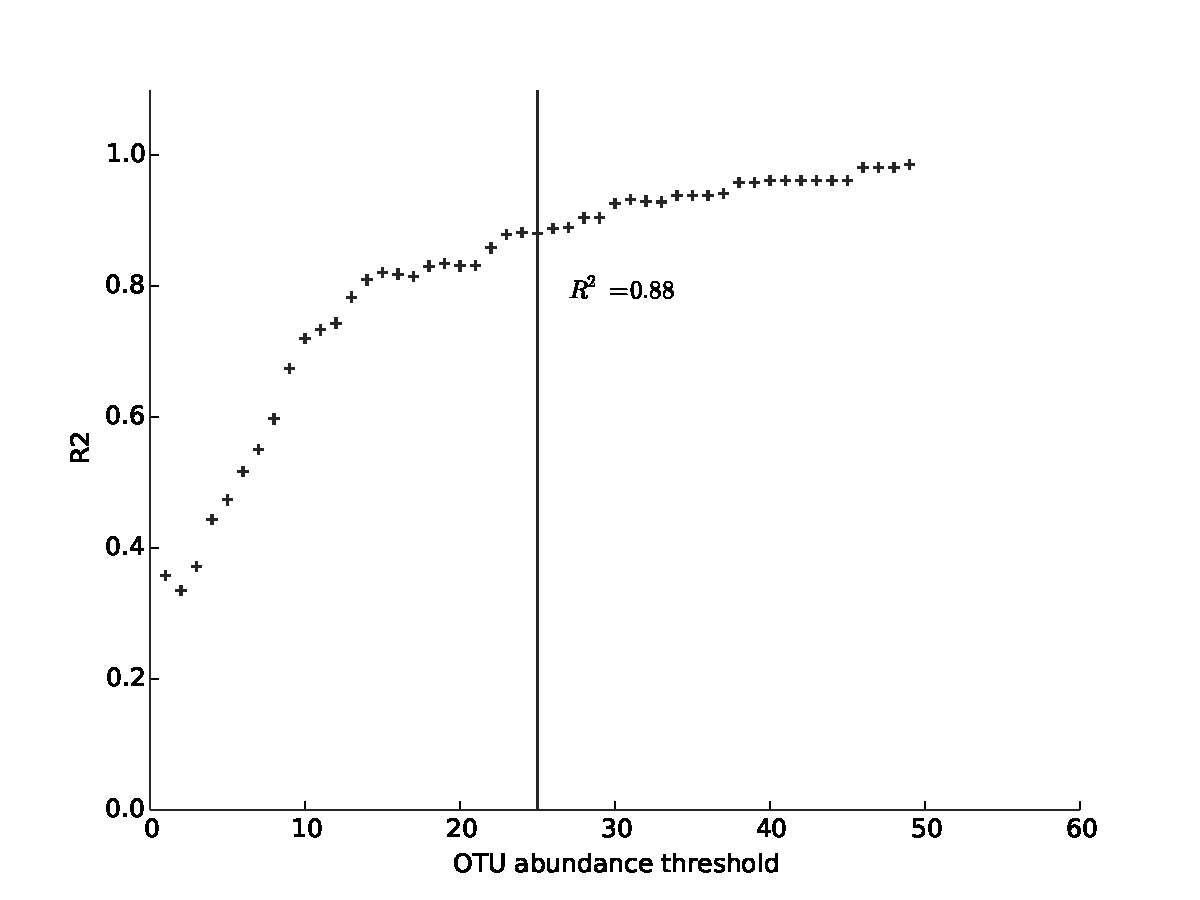
\includegraphics[width=0.8\textwidth]{figs/SB1_techrep_OTUscatR2}
  \caption[Progressive dropout analysis using log10 transformed data]{Supp. Progressive dropout analysis using log10 transformed data. X axis the threshhold of OTU abundance and y axix is the $R^2$ of linear regression of log transformed OTU abundances in two replicates when OTUs with lower abundance then threshold are discarded. When only OTUs with abundance higher than 25 are considered, $R^2$ reaches 0.88,  which is acceptable as a balance between reproducibility and data loss for low abundance OTUs within log10 transformed data.}
  \label{fig:SB1_techrep_OTUscatR2}
\end{figure}

\begin{figure}[tbph!]
  \centering
  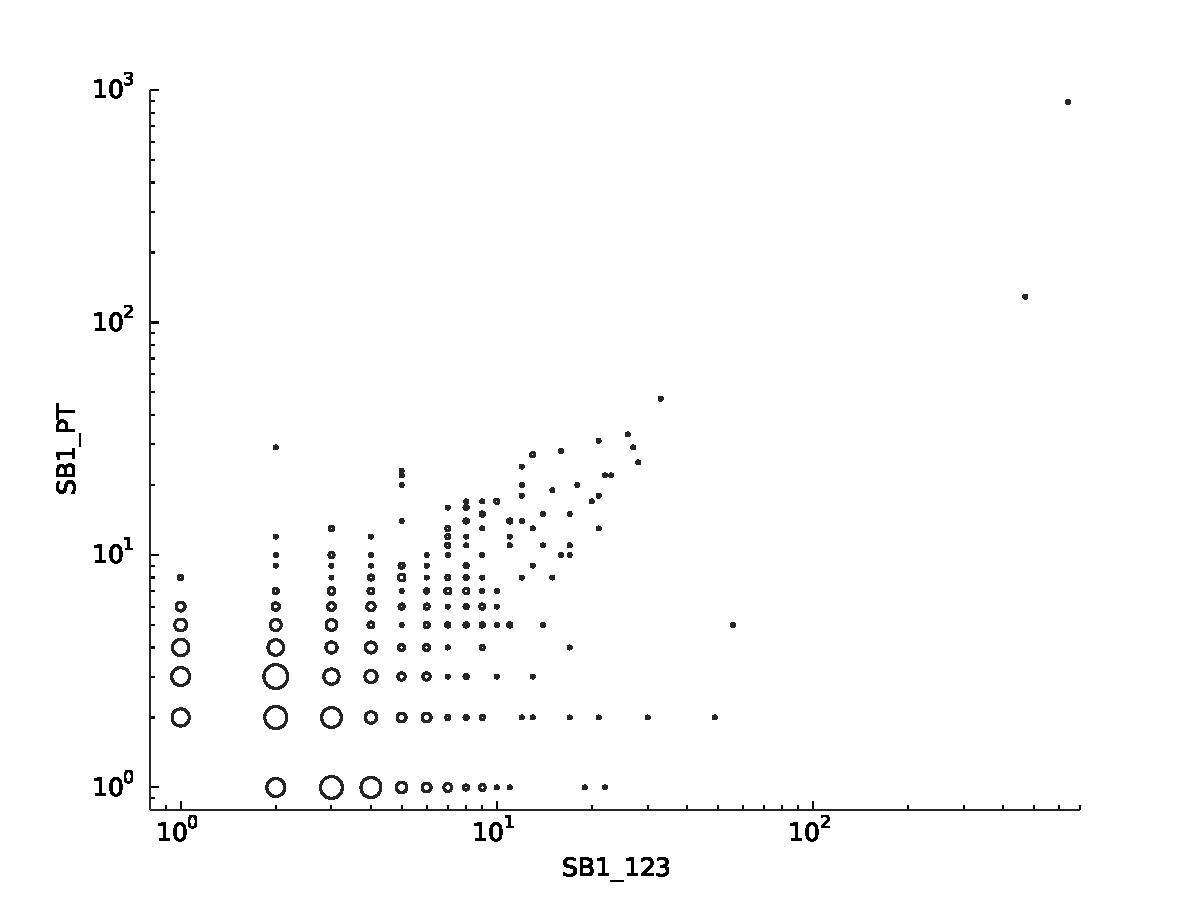
\includegraphics[width=0.8\textwidth]{figs/SB1_SGvsPT_OTUscat}
  \caption[Comparison of OTU abundance between shotgun and amplicon data in sample SB1]{Supp. Comparison of OTU abundance between shotgun and amplicon data. X axis shows number of shotgun raw reads per OTU in log scale in sample SB1, and y axis shows number of amplicon raw reads per OUT in log scale in sample SB1. The size of circle is proportional to number of OTUs with the same counts in shotgun data and also in amplicon data. The counts are in both replicates are increased by 1 to avoid 0 counts that can be displaced in log scale. There are OTUs with significant different abundance in two types of data (circles deviate from diagonal line). Peason’s correlation between two types of data is 0.873.}
  \label{fig:SB1_SGvsPT_OTUscat}
\end{figure}

\begin{figure}[tbph!]
  \centering
  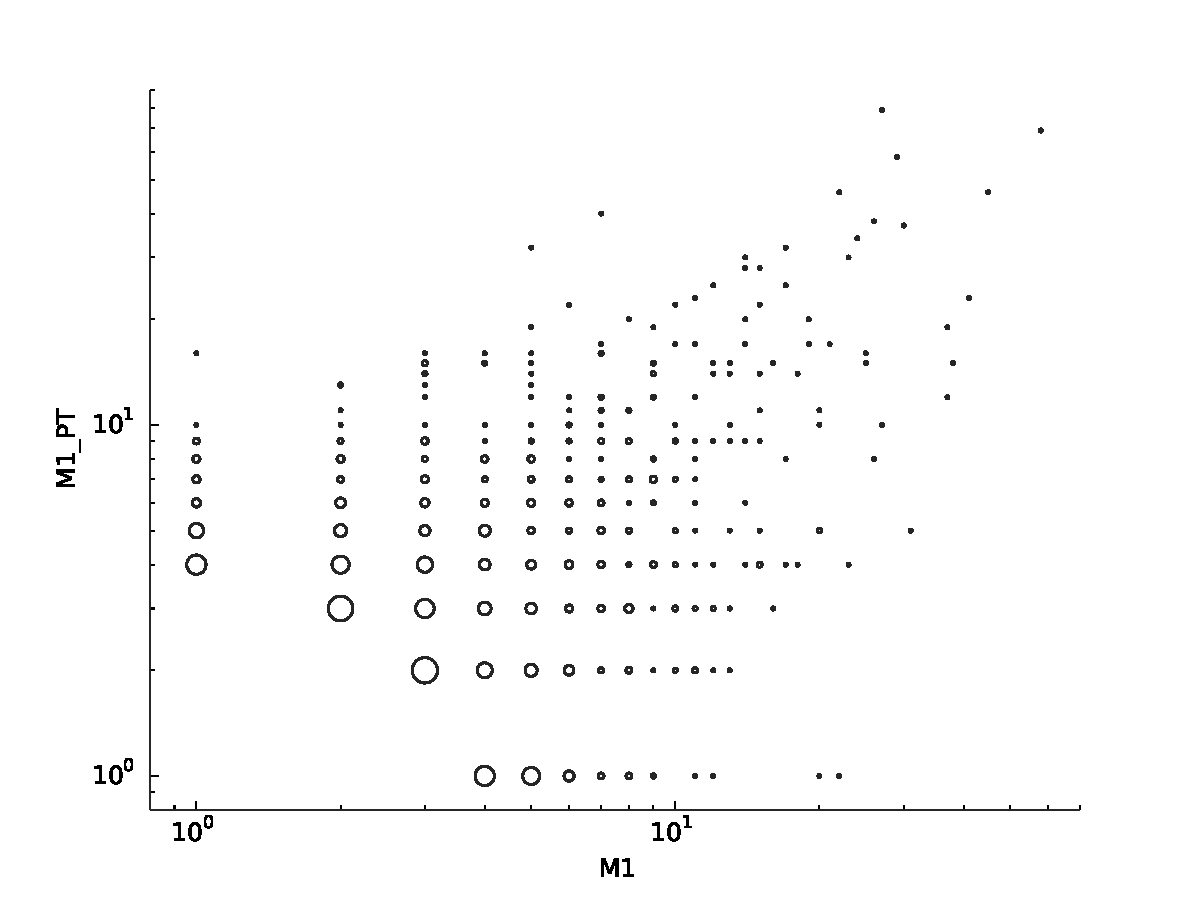
\includegraphics[width=0.8\textwidth]{figs/M1_SGvsPT_OTUscat}
  \caption[Comparison of OTU abundance between shotgun and amplicon data in sample M1. ]{Supp. Comparison of OTU abundance between shotgun and amplicon data in sample M1. X axis shows number of shotgun raw reads per OTU in log scale, and y axis shows number of amplicon raw reads per OUT in log scale. The size of circle is proportional to number of OTUs with the same counts in shotgun data and also in amplicon data. The counts are in both replicates are increased by 1 to avoid 0 counts that can be displaced in log scale. There are OTUs with significant different abundance in two types of data (circles deviate from diagonal line). Peason’s correlation between two types of data is 0.581.}
  \label{fig:M1_SGvsPT_OTUscat}
\end{figure}

  {\bf OTU based diversity analysis of shotgun SSU fragments. } 
Shotgun and amplicon data both show separation of corn and miscanthus samples, while there are also significant between these two types of data (Figure ~\ref{fig:V4_SGvsPT_pcoa}). Further, significant separation of corn and miscanthus samples is also observed when V2, V4, V6, and V8 are used for {\em de novo} OTU clustering in shotgun data (Figure ~\ref{fig:compare_vregion}). Miscanthus samples have higher diversity than corn samples in all of V2, V4, V6 and V8 regions, though variations among these regions are also observed (Figure ~\ref{fig:compare_vregion_alpha}).

\begin{figure}[tbph!]
  \centering
  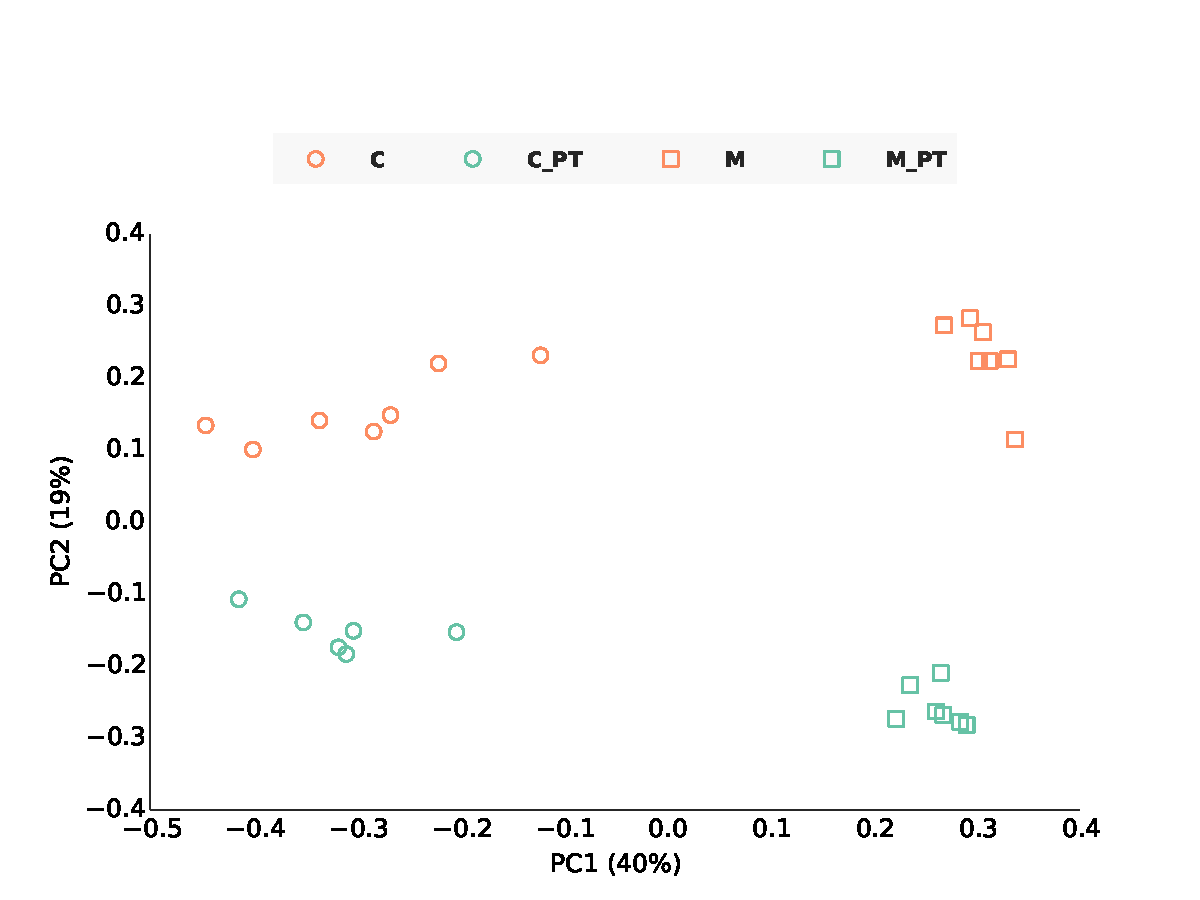
\includegraphics[width=0.8\textwidth]{figs/V4_SGvsPT_pcoa}
  \caption[PCoA of OTUs resulting from {\em de novo} clustering with shotgun data and amplicon data using 150bp of V4 region]{PCoA of OTUs resulting from {\em de novo} clustering with shotgun data and amplicon data using 150bp of V4 region. Samples with suffix ``\_PT'' (teal) are amplicon data and the others (orange) are shotgun data. Two types of data both show the separation of corn (circle) and miscanthus (square) rhizosphere samples along x-axis while there are significant differences between these two types of data shown along y-axis (AMOVA p-value < 0.01).}
  \label{fig:V4_SGvsPT_pcoa}
\end{figure}

\begin{figure}[tbph!]
  \centering
  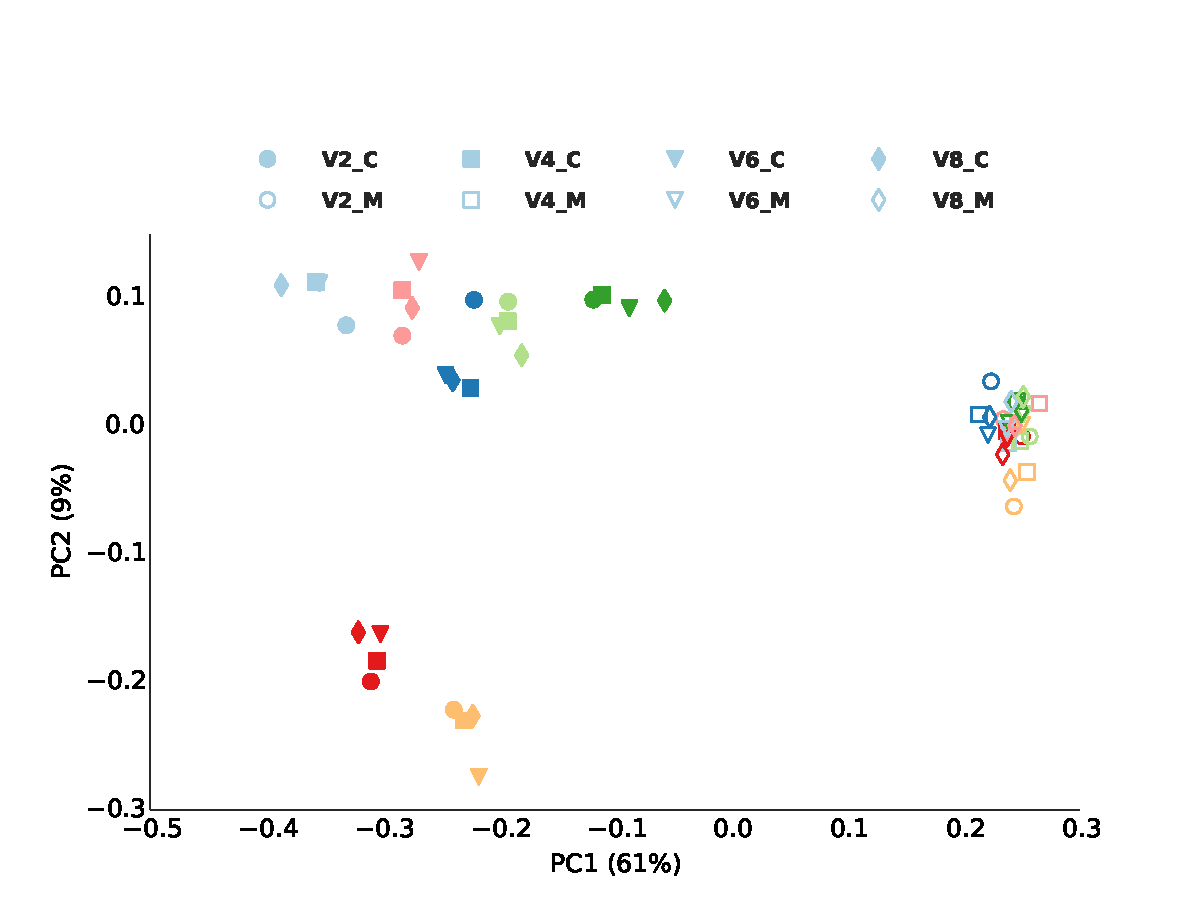
\includegraphics[width=0.8\textwidth]{figs/compare_vregion_color_1leg}
  \caption[PCoA analysis of OTUs resulting from {\em de novo} clustering with shotgun data using 150bp of V2, V4, V6, V8 regions]{Supp.?? PCoA analysis of OTUs resulting from {\em de novo} clustering with shotgun data using 150bp of V2, V4, V6, V8 regions. Different variable regions in the shotgun data can be used for clustering and show the same grouping of samples, which is separation of corn (filled markers) and miscanthus (unfilled markers) rhizosphere samples along x-axis. The PCoA results of different variable regions are plotted together using procrutes analysis in QIIME.}
  \label{fig:compare_vregion}
\end{figure}

\begin{figure}[tbph!]
  \centering
  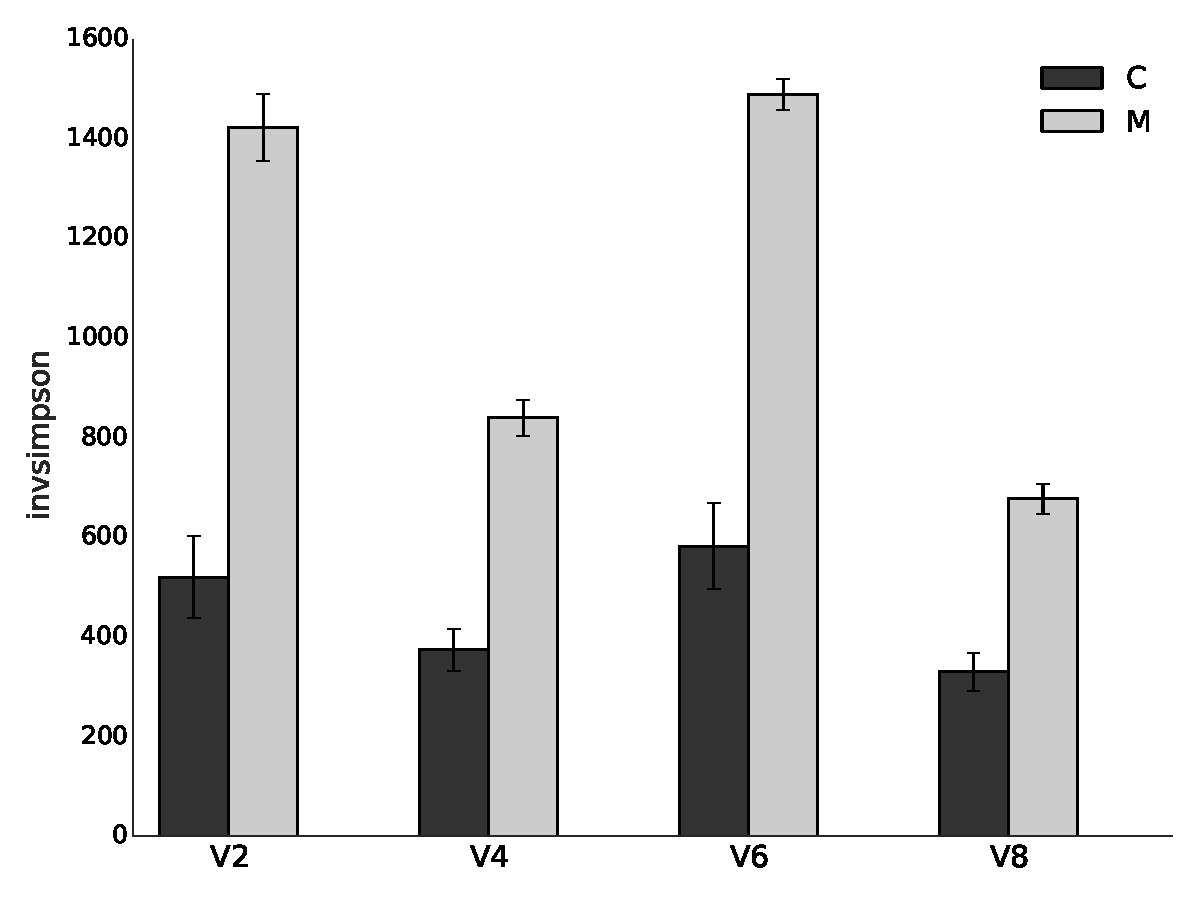
\includegraphics[width=0.8\textwidth]{figs/compare_vregion_alpha.pdf}
  \caption[Alpha diversity of OTUs resulting from {\em de novo} clustering with shotgun data using 150bp of V2, V4, V6, V8 regions]{Alpha diversity of OTUs resulting from {\em de novo} clustering with shotgun data using 150bp of V2, V4, V6, V8 regions. All variable regions show M (miscanthus) is more diverse than C (corn), even though there are variation of diversity among regions.}
  \label{fig:compare_vregion_alpha}
\end{figure}

  {\bf Copy corretion. }
  Both soil samples (SB1 and M1) show firmicutes and bacteroidetes have highest fold change after copy correction. Especially for firmicutes, its fold change (about 3) is much higher than the rest (Figure ~\ref{fig:SB1+M1_cc}). Despite of the relative abundance change after copy correction, grouping pattern of our soils samples does not change.

\begin{figure}[tbph!]
  \centering
  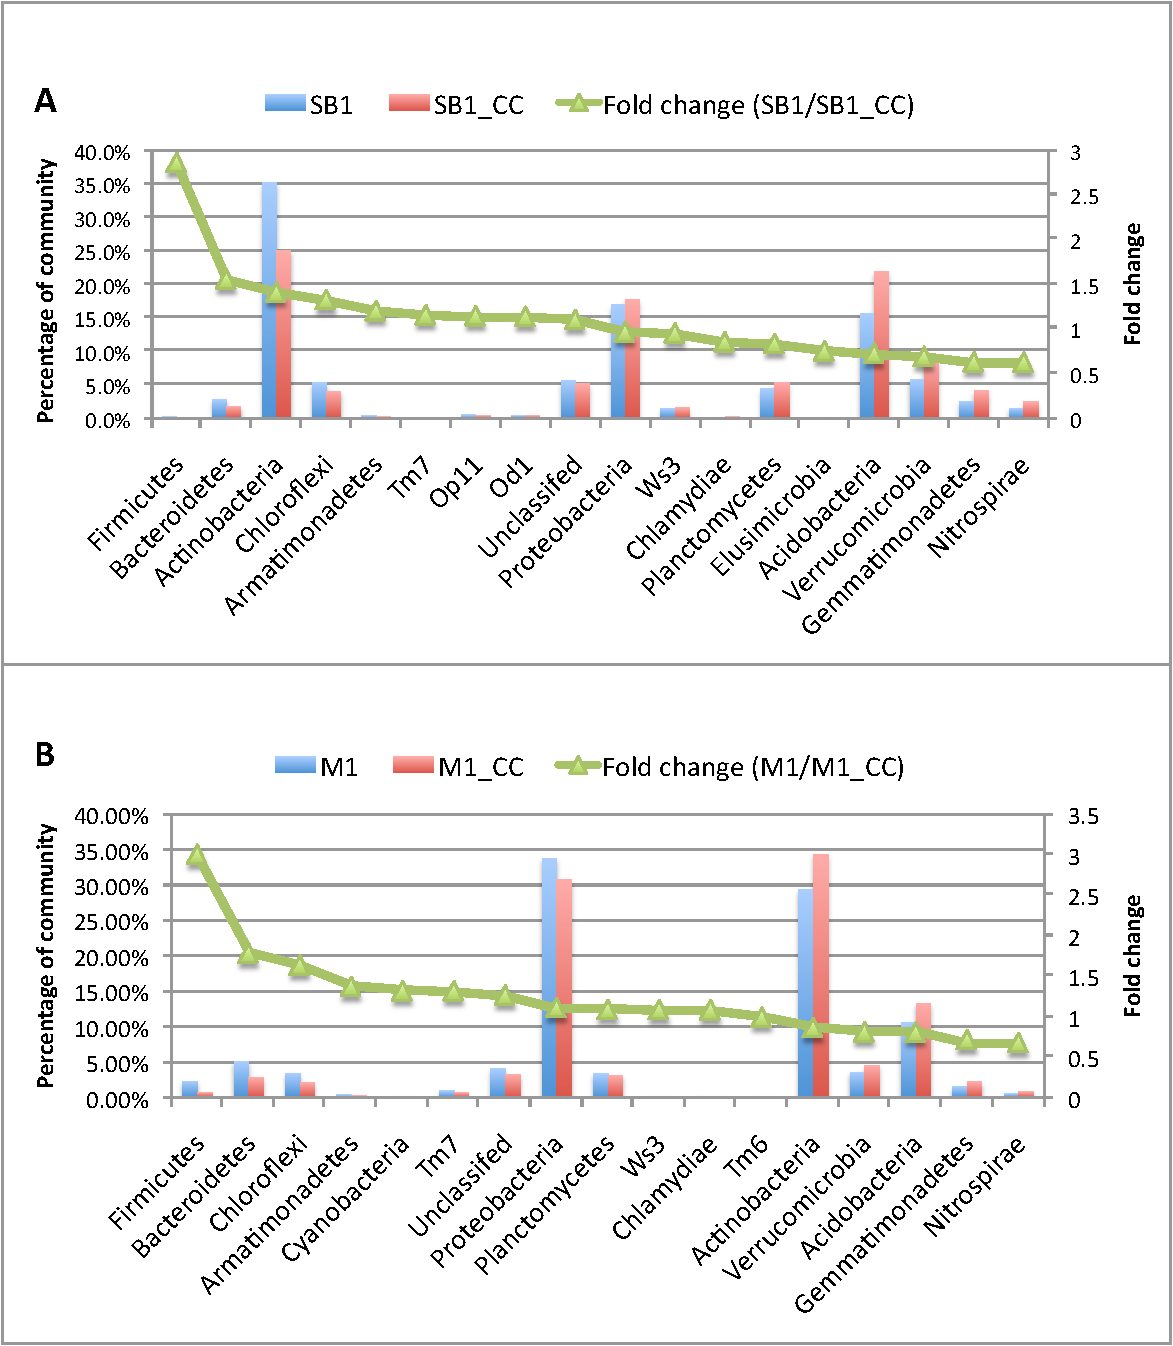
\includegraphics[width=0.8\textwidth]{figs/SB1+M1_cc}
  \caption[Taxonomy summary before and after SSU rRNA gene copy correction]{Bacterial phylum level taxonomy summary before and after SSU rRNA gene copy correction. Left vertical axis shows percentage in total community and right vertical axis shows fold change after copy correction. Taxon with relative abundance of more than 0.1\% before copy correction are chosen and are ordered based on fold change.}
  \label{fig:SB1+M1_cc}
\end{figure}

\section{Discussion}
  We present, characterize and validate an efficient method for mining and analyzing SSU rRNA genes from shotgun metagenomic sequence that has advantages over existing shotgun analysis pipelines such as MG-RAST. MG-RAST annotates shotgun reads by BLAT search against rRNA databases and taxonomy of reads is inferred from the best hit or least common ancestor of several top hits (\cite{blast,blat,mgrast}), but BLAT or BLAST-like tools are too slow for large dataset and thus only applicable when run in parallel in computer clusters. Moreover, these pipelines lacks the OTU based community analysis.

  HMM based rRNA gene search has been applied extensively (\cite{metarna,rrnaselector,metaxa}). The main improvement we made is on search speed. While other tools built separate model for Bacteria, Archaea, and Eukarya, we use one model for Bacteria and Archaea built from well-curated SILVA reference sequences. Testing results show that this model is sufficient to cover 99.3\% of the search results (29747 out of 29959 at default e-value cutoff of 10) by all the models in metaxa, because SSU rRNA genes are conserved and the combined model still has high sensitivity when loose e-value cutoff is used. Since this step is the computation bottleneck, we can get great speed improvement by searching with only two HMMs (one for Bacteria and Archaea and one for Eukaryota) instead of three (one for each domain). The search results can be further classified into domains or even species using classifier. Moreover, false positives are tolerable in this initial search step since there is a filtering step next. Since this analysis focus on diversity analysis, the search step is optional and the SSU rRNA fragments identified by other tools can also be fed directly to the following steps.

    Then a Nearest Alignment Space Termination (NAST) (\cite{mothuraligner2009}) based alignment method implemented in Mothur is used for aligning the SSU fragments and screening false positives by the their identity to the most similar reference in reference set provided in Mothur. The choice of identity cutoff (50\%) is arbitrary here, since there is no clear definition of SSU rRNA gene and those reads with low identity to reference sequences are also discard prio to clustering in traditional amplicon analysis pipelines (\cite{rdp2009, mothur, qiime}). Meanwhile amplicon sequences with less than 50\% to reference sequences are also discarded for consistency in comparison. An alignment of the SSU rRNA gene fragments is essential for the later {\em de novo} OTU related analysis. Compared to the methods that use only the 16S rRNA gene in E.coli as alignment template (\cite{kostas2013}), this method takes advantages of the rich phylogenetic diversity of SSU rRNA genes provided by SILVA database. Increasing the number of reference sequences included can improve the quality of alignment, but also linearly increases the memory required (\cite{mothuraligner2009,pynast}).

  Our pipeline also integrates RDP classifier that is suitable for classification of reads as short as 50bp (\cite{rdpclassifier}). In taxonomy comparison of shotgun and amplicon data, two main SSU rRNA gene database, RDP and SILVA, are used to make sure the taxonomy distribution is not caused by reference database. In addition, LSU rRNA gene is also used to confirm the classification by SSU rRNA gene. V6-V8 primer set shows significant bias against Verrucomicrobia, consistent with other studies showing that Verrucomicrobia’s abundance in soil samples is underestimated due to primer bias (\cite{verruco2011}). In contrary, V4 primer set shows bias to Verrucomicrobia. This result agrees with studies showing that V4 primer set has better coverage of Verrucomicrobia (\cite{verruco2011}). Further, V4 primer sets shows bias against Actinobacteria. The V4 primer set is reported cover 92.43\% of Actinobacteria in reference databases, the lowest among nine common bacterial phyla (Verrucomicrobial, Acidobacteria, Actinobacteria, Bacteriodetes, Chloroflexi, Firmicutes, Gemmatimonadetes, Planctomycetes, and Proteobactera) (\cite{verruco2011}). Primer bias against Actinobacteria has also been reported in environmental samples using a Sanger sequencing primer (24F/1492R) (\cite{actinobias}). V4 primer set (515F/806R) remains a good choice as universal primers due to its overall coverage of bacterial phyla, but attentions need to be paid to the missing Actinobacteria in future studies, especially if they are interest groups in a study.

  Gene copy number is another source of bias that limit our ability to find accurate microbial community profile. There are up to 15 SSU rRNA gene copy in Bacteria and up to 5 in Archaea (\cite{rrncopy2004}). This pipeline utilizes SSU rRNA copy database in CopyRighter (\cite{copyrighter}). Both of our testing soil samples shows firmicutes has highest fold change (Figure ~\ref{fig:SB1+M1_cc}), consistent with finding in CopyRighter paper (\cite{copyrighter}). Even thought gene copy corrention changes the absolute and relative abundance most OTU or taxon, grouping pattern of our soil samples in ordination analysis is still the same as before copy correction. Copy correction is still an open problem due to facts that SSU rRNA gene copy number for most speices are lacking and copy number can be incorrect for species with complete genome sequences because of mis-assembly of these repeated regions. It might be OK to skip copy correction when comparing communities using data targeting the same gene, because the copy number bias can be treated as systematic bias. However, copy correction is necessary when different data are used. (e.g. comparing community profiles using SSU rRNA gene amplicon data and using annotation from all of whole genome shotgun data.)

  Generally, OTU based analysis provides higher resolution than taxonomy (\cite{patotuasse2011}) based diversity analysis for community comparison, mainly due to lack of reference sequence from unculturable microbes in the databases. The high correlation of OTU abundance in two technical replicates shows the reproducibility shotgun data. Moreover, Pearson’s correlation coefficient of log-transformed OTU abundance in two replicates increased from 0.584 to 0.938 after OTUs with abundance lower than 25 are discarded. Consistently, $R^2$ of linear regression between log-transformed OTU abundance reaches 0.88 after removing OTUs with abundance lower than 25, which is comparable to the reproducibility of amplicon data mentioned in \cite{arabdopsis}. Further, comparison of OTU abundance in shotgun data and amplicon data sequenced from the same DNA extraction also show many OTUs have inconsistent abundance in two types of data, which agrees with the difference seen in the taxonomy based comparison.

  The beta-diversity analysis by ordination methods such as PCoA and NMDS is one of the most common analyses in microbial ecology. To the best of our knowledge, the methods used in \cite{kostas2013,phylotu} are the only existing tools that are designed to deal with {\em de novo} clustering of Illumina shotgun reads. The former could results in bad alignment by using only 16S rRNA gene in E.coli as alignment template. The latter (PhylOTU) does the OTU clustering of SSU rRNA gene fragments aligned together over whole gene length, which can be problematic because fragments aligned to different regions do not overlap and thus the clustering results are not reliable, even though the reference sequences included in the clustering process can improve the results. In our clustering method, we make sure all the sequences overlap by picking one small region (150bp) and all sequences included in clustering have lengths longer than 100bp. In addition, we got longer reads by assembling overlapping pair end reads (Figure ~\ref{fig:read_length_dist}) and longer reads can make sure more reads overlap and thus suitable for {\em de novo} clustering. Further, several studies have shown 150bp in a variable region produce very similar PCoA results to 400bp in the same variable regions (\cite{robknight2007,caporaso2012miseq}). As read lengths increase with improvement of sequencing technology, longer regions can be chosen and the clustering results will be even more reliable. Further, shotgun data give us the flexibility of choose any variable region (Figure ~\ref{fig:compare_vregion}) and consistency of results from different variable region gives us more confidence on the biological conclusion and the method itself.

  In this study, LSU rRNA gene is used mainly as confirmation analysis for SSU rRNA gene based diversity analysis. However, LSU rRNA gene offers additional stretches of variable and characteristic sequence regions due to longer sequence length, and thus better phylogenetic resolution (\cite{lsuprimer}). For the above reason and also another reason that there are more available references for fungi, LSU rRNA gene is commonly used for fungal community studies (\cite{lsufungal2007,lsuclassifier,lsufungal2012,lsufungal2010}). As a universal marker gene, LSU rRNA gene is limited by reference sequences and universal primer sets available (\cite{lsuprimer}). The limitation of the references is confirmed by more unclassified sequences by LSU rRNA than SSU rRNA gene (Figure ~\ref{fig:V6to8_SB1_taxa},~\ref{fig:V4_M1_taxa}). This analysis framework provides a way to avoid the primer limitation and bias for LSU rRNA gene. The consistency of SSU rRNA gene and LSU rRNA gene taxonomy profiles at domain and bacteria phylum level of the same sample shown in this study is promising evidence. With increasing reference sequences in database and improved manly-curated alignment, LSU rRNA gene would be as good marker gene as SSU rRNA gene. Further, comparison between both genes and across multiple regions can provide cross validation and thus help us make solid conclusion (Figure ~\ref{fig:compare_vregion}).

\section{Conclusion}
Although shotgun sequencing has its advantages such as no chimera and primer bias, analyzing big data has been a big challenge. In this study, an efficient method for searching and analyzing SSU rRNA fragments was developed. It takes advantage of HMMER for searching SSU rRNA gene and LSU rRNA gene from Bacteria, Archaea and Eukaryota, and can be run on most desktops with more than 4Gb memory (the memory is for loading all reference sequences for alignment). Since SSU rRNA based community analysis is an important tool in microbial ecology, this method can save projects already done shotgun sequencing from additional cost of SSU rRNA amplicon sequencing. As read length and sequencing depth increases, longer and more SSU rRNA gene fragments can be recovered. Thus clustering and beta-diversity analysis will become even more reliable. In addition, we have shown LSU rRNA has very consistent with SSU rRNA gene in terms of taxonomy. In future, other single copy genes such as {\em rpoB}, {\em gyrB}, and {\em recA} can also be recovered and used for community structure analysis, as more resolving complements for current main stream of SSU/LSU rRNA based analysis.

\bibliographystyle{unsrt}
\bibliography{refs.bib}

\section{Supplements}

    \begin{figure}[tbph!]
    \centering
    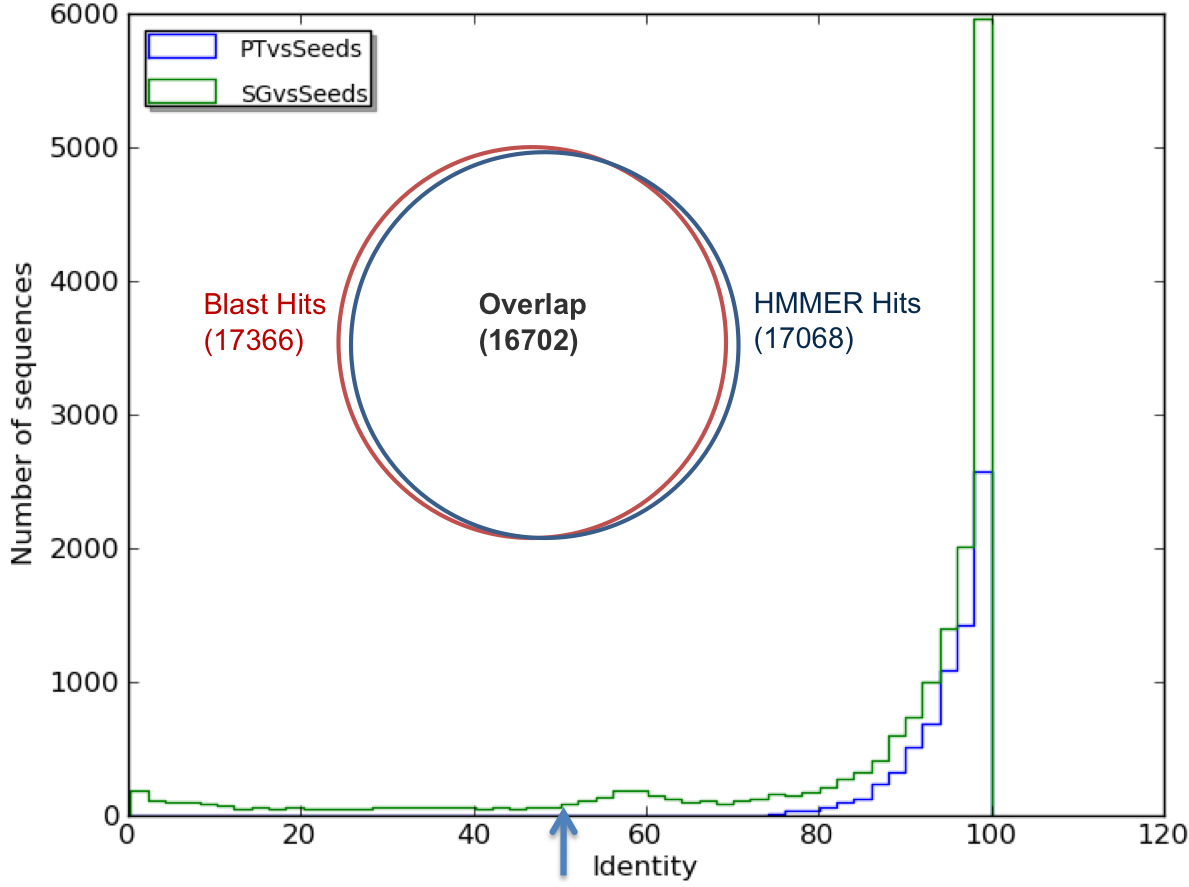
\includegraphics[width=0.8\textwidth]{figs/vennPlusIdenDisWholeLength}
    \caption[Venn diagram of BLAST and HMMER hits and pairwise identity distribution to the reference SSU rRNA genes]{Venn diagram of BLAST and HMMER hits and pairwise identity distribution to the reference SSU rRNA genes. BLAST and HMMER was ran with e-value cutoff of $10^{-5}$ and $10$ respectively.}
    \label{fig:vennPlusIdenDisWholeLength}
    \end{figure}


\end{document}
